% Practice Test 04 — Minnesota Edition
% Questions: 30 (21 MC + 9 SA)
% Generated by scripts/generate_practice_tests.py

\begin{practiceQuestion}{1-3-q06}{mc}
\begin{questionText}
On a proportional graph, the point $(1, r)$ represents:
\end{questionText}
\choiceA{The $x$-intercept}
\choiceB{The constant of proportionality}
\choiceC{The slope of the line}
\choiceD{Both B and C}
\correctAnswer{D}
\explanation{At $x = 1$, $y = k \times 1 = k$. So the point $(1, r)$ gives the constant of proportionality, which is also the slope.}
\end{practiceQuestion}

\begin{practiceQuestion}{1-5-q06}{mc}
\begin{questionText}
Runner A passes through $(2, 10)$ and Runner B passes through $(2, 8)$. Both start at $(0, 0)$. Who is faster?
\end{questionText}
\choiceA{Runner A}
\choiceB{Runner B}
\choiceC{They are the same speed}
\choiceD{Cannot be determined}
\correctAnswer{A}
\explanation{Runner A: $k = \frac{10}{2} = 5$. Runner B: $k = \frac{8}{2} = 4$. A higher $k$ means faster speed, so Runner A is faster.}
\end{practiceQuestion}

\begin{practiceQuestion}{1-6-q04}{mc}
\begin{questionText}
A recipe for $4$ people uses $\frac{3}{2}$ cups of rice. How much rice is needed for $10$ people?
\end{questionText}
\choiceA{$2\frac{1}{2}$ cups}
\choiceB{$3$ cups}
\choiceC{$3\frac{3}{4}$ cups}
\choiceD{$5$ cups}
\correctAnswer{C}
\explanation{Per person: $\frac{3}{2} \div 4 = \frac{3}{8}$ cup. For $10$: $\frac{3}{8} \times 10 = \frac{30}{8} = 3\frac{3}{4}$ cups.}
\end{practiceQuestion}

\begin{practiceQuestion}{2-1-q11}{mc}
\begin{questionText}
A baker made $120$ cupcakes and sold $90$ of them. What percent of the cupcakes were sold?
\end{questionText}
\choiceA{$60\%$}
\choiceB{$70\%$}
\choiceC{$75\%$}
\choiceD{$80\%$}
\correctAnswer{C}
\explanation{Divide: $90 \div 120 = 0.75 = 75\%$.}
\end{practiceQuestion}

\begin{practiceQuestion}{2-5-q13}{mc}
\begin{questionText}
A delivery app charges a $\$3$ flat fee plus a $10\%$ service fee on your order. If your order is $\$30$, what is the total?


\numberLine[5]{0}{35}
\end{questionText}
\choiceA{$\$33.00$}
\choiceB{$\$33.30$}
\choiceC{$\$36.00$}
\choiceD{$\$36.30$}
\correctAnswer{C}
\explanation{Service fee: $30 \times 0.10 = \$3$. Total: $30 + 3 + 3 = \$36$.}
\end{practiceQuestion}

\begin{practiceQuestion}{2-7-q24}{sa}
\begin{questionText}
You guessed there were $300$ people at a concert. The actual attendance was $350$. Find the percent error (rounded to the nearest tenth).
\end{questionText}
\correctAnswer{$\approx 14.3\%$}
\explanation{$\frac{|300 - 350|}{350} \times 100 = \frac{50}{350} \times 100 \approx 14.3\%$.}
\end{practiceQuestion}

\begin{practiceQuestion}{2-8-q28}{gmc}
\begin{questionText}
The bar graph shows interest earned on a $\$1{,}000$ deposit at three different banks after $1$ year. Which bank pays the highest interest rate?

\begin{center}
\begin{tikzpicture}[scale=0.7]
  \draw[thick,->] (0,0) -- (0,5) node[above] {Interest (\$)};
  \draw[thick,->] (0,0) -- (8,0);
  \foreach \y/\label in {0/0, 1/10, 2/20, 3/30, 4/40} {
    \draw (-0.1,\y) -- (0.1,\y);
    \node[left] at (-0.15,\y) {\footnotesize \$\label};
  }
  % Bank X
  \fill[funBlue!70] (0.5,0) rectangle (2,2);
  \node[below] at (1.25,0) {\footnotesize Bank X};
  \node[above] at (1.25,2) {\footnotesize \$20};
  % Bank Y
  \fill[funRed!70] (3,0) rectangle (4.5,3.5);
  \node[below] at (3.75,0) {\footnotesize Bank Y};
  \node[above] at (3.75,3.5) {\footnotesize \$35};
  % Bank Z
  \fill[green!50!black] (5.5,0) rectangle (7,1.5);
  \node[below] at (6.25,0) {\footnotesize Bank Z};
  \node[above] at (6.25,1.5) {\footnotesize \$15};
\end{tikzpicture}
\end{center}
\end{questionText}
\choiceA{Bank X}
\choiceB{Bank Y}
\choiceC{Bank Z}
\choiceD{They all pay the same}
\correctAnswer{B}
\explanation{Bank Y earned $\$35$ on $\$1{,}000$, which is $3.5\%$ — the highest of the three.}
\end{practiceQuestion}

\begin{practiceQuestion}{3-1-q25}{sa}
\begin{questionText}
Which integer is $5$ units to the left of $2$ on the number line?
\end{questionText}
\correctAnswer{$-3$}
\explanation{Moving $5$ units left from $2$: $2 - 5 = -3$.}
\end{practiceQuestion}

\begin{practiceQuestion}{4-1-q02}{mc}
\begin{questionText}
What is the value of $3x - 5$ when $x = 4$?
\end{questionText}
\choiceA{$2$}
\choiceB{$7$}
\choiceC{$17$}
\choiceD{$-2$}
\correctAnswer{B}
\explanation{Substitute: $3(4) - 5 = 12 - 5 = 7$.}
\end{practiceQuestion}

\begin{practiceQuestion}{4-2-q27}{gmc}
\begin{questionText}
The lengths of the four sides of a quadrilateral are shown below. What is the simplified perimeter?

\begin{center}
\begin{tikzpicture}[scale=0.9]
  \draw[thick, fill=funBlue!10] (0,0) -- (4,0) -- (5,3) -- (1,3) -- cycle;
  \node[below] at (2,0) {$3x + 2$};
  \node[right] at (4.7,1.5) {$x + 1$};
  \node[above] at (3,3) {$2x - 3$};
  \node[left] at (0.3,1.5) {$x + 4$};
\end{tikzpicture}
\end{center}
\end{questionText}
\choiceA{$7x + 4$}
\choiceB{$6x + 4$}
\choiceC{$7x - 4$}
\choiceD{$6x + 10$}
\correctAnswer{A}
\explanation{Add all sides: $(3x + 2) + (x + 1) + (2x - 3) + (x + 4)$. Combine variable terms: $3x + x + 2x + x = 7x$. Combine constants: $2 + 1 - 3 + 4 = 4$. Perimeter: $7x + 4$.}
\end{practiceQuestion}

\begin{practiceQuestion}{5-2-q05}{mc}
\begin{questionText}
Solve $14 = 2m + 6$.
\end{questionText}
\choiceA{$m = 4$}
\choiceB{$m = 10$}
\choiceC{$m = 8$}
\choiceD{$m = 3$}
\correctAnswer{A}
\explanation{Subtract $6$: $8 = 2m$. Divide by $2$: $m = 4$. Check: $2(4) + 6 = 14$ \checkmark.}
\end{practiceQuestion}

\begin{practiceQuestion}{5-3-q29}{gsa}
\begin{questionText}
The total area of the figure below is $84$ square cm. Find $x$.

\begin{center}
\begin{tikzpicture}[scale=0.5]
  % 6 identical rectangles side by side
  \foreach \i in {0,...,5} {
    \draw[thick,fill=funBlue!15] (\i*2,0) rectangle (\i*2+2,3);
  }
  \draw[<->] (0,-0.7) -- (12,-0.7);
  \node[below] at (6,-0.7) {$6$ rectangles, each width $(x + 1)$ cm};
  \draw[<->] (-0.7,0) -- (-0.7,3);
  \node[left] at (-0.7,1.5) {$2$ cm};
  \node at (6,4.2) {Total area $= 84$ sq. cm};
\end{tikzpicture}
\end{center}
\end{questionText}
\correctAnswer{$x = 6$}
\explanation{Total area $= 6 \times 2 \times (x + 1) = 84$. So $12(x + 1) = 84$. Divide by $12$: $x + 1 = 7$. Subtract $1$: $x = 6$.}
\end{practiceQuestion}

\begin{practiceQuestion}{5-4-q26}{gmc}
\begin{questionText}
The table shows input and output values for a function. What is the rule?

\begin{center}
\begin{tabular}{|c|c|}
\hline
\textbf{Input ($x$)} & \textbf{Output ($y$)} \\
\hline
$2$ & $2.5$ \\
\hline
$4$ & $3.5$ \\
\hline
$6$ & $4.5$ \\
\hline
$10$ & $6.5$ \\
\hline
\end{tabular}
\end{center}
\end{questionText}
\choiceA{$y = 0.5x + 1.5$}
\choiceB{$y = x - 0.5$}
\choiceC{$y = 0.25x + 2$}
\choiceD{$y = 2x - 1.5$}
\correctAnswer{A}
\explanation{From $x = 2$ to $x = 4$, $y$ increases by $1$ while $x$ increases by $2$, so rate $= 0.5$. When $x = 2$: $0.5(2) + 1.5 = 2.5$ \checkmark.}
\end{practiceQuestion}

\begin{practiceQuestion}{5-5-q13}{mc}
\begin{questionText}
Which value of $x$ is a solution to $4x - 1 > 11$?
\end{questionText}
\choiceA{$x = 2$}
\choiceB{$x = 3$}
\choiceC{$x = 4$}
\choiceD{$x = 1$}
\correctAnswer{C}
\explanation{Solve: $4x > 12$, so $x > 3$. Only $x = 4$ satisfies $x > 3$. Check: $4(4) - 1 = 15 > 11$ \checkmark.}
\end{practiceQuestion}

\begin{practiceQuestion}{5-6-q13}{mc}
\begin{questionText}
True or false: The graph of $x < 5$ and $x \leq 5$ look exactly the same.
\end{questionText}
\choiceA{True — both shade to the left of $5$}
\choiceB{False — $x < 5$ has an open circle, $x \leq 5$ has a closed circle}
\choiceC{False — they shade in different directions}
\choiceD{True — the circle type does not matter}
\correctAnswer{B}
\explanation{$x < 5$ uses an open circle (not including $5$) while $x \leq 5$ uses a closed circle (including $5$). Both shade left.}
\end{practiceQuestion}

\begin{practiceQuestion}{6-3-q15}{mc}
\begin{questionText}
Which condition makes it impossible to draw a triangle?
\end{questionText}
\choiceA{Sides $5$, $12$, $13$}
\choiceB{Sides $7$, $7$, $7$}
\choiceC{Sides $1$, $1$, $3$}
\choiceD{Sides $8$, $15$, $17$}
\correctAnswer{C}
\explanation{$1 + 1 = 2 < 3$. The triangle inequality fails. The other three sets all satisfy the triangle inequality.}
\end{practiceQuestion}

\begin{practiceQuestion}{6-4-q19}{sa}
\begin{questionText}
Two angles of a triangle are $72°$ and $53°$. What is the third angle?
\end{questionText}
\correctAnswer{$55°$}
\explanation{$180° - 72° - 53° = 55°$.}
\end{practiceQuestion}

\begin{practiceQuestion}{6-5-q27}{gmc}
\begin{questionText}
The diagram shows a cone being sliced. Which cut produces a circular cross-section?

\begin{center}
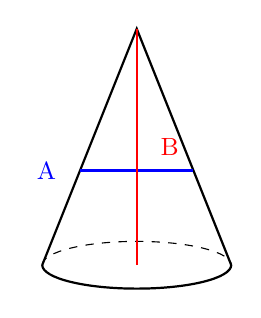
\begin{tikzpicture}[scale=0.6]
  % Cone
  \draw[thick] (-2,0) -- (0,5) -- (2,0);
  \draw[thick] (-2,0) arc[start angle=180,end angle=360,x radius=2,y radius=0.5];
  \draw[dashed] (-2,0) arc[start angle=180,end angle=0,x radius=2,y radius=0.5];
  % Cut A - horizontal
  \draw[thick,blue] (-1.2,2) -- (1.2,2);
  \node[left,blue] at (-1.5,2) {\small A};
  % Cut B - vertical through apex
  \draw[thick,red] (0,0) -- (0,5);
  \node[right,red] at (0.3,2.5) {\small B};
\end{tikzpicture}
\end{center}
\end{questionText}
\choiceA{Cut A (horizontal)}
\choiceB{Cut B (vertical through apex)}
\choiceC{Both cuts}
\choiceD{Neither cut}
\correctAnswer{A}
\explanation{Cut A (horizontal, parallel to the base) produces a circle. Cut B (vertical through the apex) produces a triangle.}
\end{practiceQuestion}

\begin{practiceQuestion}{6-6-q24}{sa}
\begin{questionText}
Three angles meet at a point on a line: $50°$, $(2x + 10)°$, and $x°$. Find $x$.
\end{questionText}
\correctAnswer{$40$}
\explanation{Angles on a line sum to $180°$: $50 + 2x + 10 + x = 180$. Combine: $3x + 60 = 180$. Solve: $3x = 120$, $x = 40$.}
\end{practiceQuestion}

\begin{practiceQuestion}{7-3-q01}{mc}
\begin{questionText}
What is the area of a circle with a radius of $3$ cm? Use $\pi \approx 3.14$.
\end{questionText}
\choiceA{$9.42$ cm$^2$}
\choiceB{$18.84$ cm$^2$}
\choiceC{$28.26$ cm$^2$}
\choiceD{$113.04$ cm$^2$}
\correctAnswer{C}
\explanation{$A = \pi r^2 = 3.14 \times 3^2 = 3.14 \times 9 = 28.26$ cm$^2$.}
\end{practiceQuestion}

\begin{practiceQuestion}{7-4-q02}{mc}
\begin{questionText}
What is the first step to find the area of a composite shape?
\end{questionText}
\choiceA{Multiply all the side lengths}
\choiceB{Break it into simpler shapes}
\choiceC{Find the perimeter first}
\choiceD{Measure the diagonal}
\correctAnswer{B}
\explanation{To find the area of a composite shape, break it into simpler shapes (rectangles, triangles, circles, etc.), find each area, and then add or subtract.}
\end{practiceQuestion}

\begin{practiceQuestion}{7-5-q15}{mc}
\begin{questionText}
A triangular prism has two triangular bases each with area $15$ cm$^2$. The three rectangular lateral faces have areas $40$ cm$^2$, $30$ cm$^2$, and $50$ cm$^2$. What is the total surface area?
\end{questionText}
\choiceA{$120$ cm$^2$}
\choiceB{$135$ cm$^2$}
\choiceC{$150$ cm$^2$}
\choiceD{$165$ cm$^2$}
\correctAnswer{C}
\explanation{Two bases: $2 \times 15 = 30$ cm$^2$. Lateral faces: $40 + 30 + 50 = 120$ cm$^2$. Total: $30 + 120 = 150$ cm$^2$.}
\end{practiceQuestion}

\begin{practiceQuestion}{7-6-q21}{sa}
\begin{questionText}
A triangular prism has a triangular base with base $10$ m and height $6$ m. The prism is $8$ m long. What is the volume?
\end{questionText}
\correctAnswer{$240$ m$^3$}
\explanation{$B = \frac{1}{2} \times 10 \times 6 = 30$ m$^2$. $V = 30 \times 8 = 240$ m$^3$.}
\end{practiceQuestion}

\begin{practiceQuestion}{8-1-q03}{mc}
\begin{questionText}
Which sampling method is most likely to produce a representative sample of a school's students?
\end{questionText}
\choiceA{Survey students in the cafeteria during lunch}
\choiceB{Survey every fifth student on an alphabetical class list}
\choiceC{Survey students who volunteer to participate}
\choiceD{Survey only students in honors classes}
\correctAnswer{B}
\explanation{Selecting every fifth student from a list is systematic and gives all students an equal chance, making it more representative.}
\end{practiceQuestion}

\begin{practiceQuestion}{8-3-q21}{sa}
\begin{questionText}
Data set: $4, 6, 7, 8, 10$. The mean is $7$. Find the MAD.
\end{questionText}
\correctAnswer{$1.6$}
\explanation{Deviations from mean: $|4-7|+|6-7|+|7-7|+|8-7|+|10-7| = 3+1+0+1+3 = 8$. MAD $= \frac{8}{5} = 1.6$.}
\end{practiceQuestion}

\begin{practiceQuestion}{8-4-q24}{sa}
\begin{questionText}
Explain one advantage of using IQR instead of range to describe the spread of a data set.
\end{questionText}
\correctAnswer{IQR is not affected by outliers}
\explanation{Range uses only the extreme values, which can be misleading with outliers. IQR measures the middle $50\%$ and gives a more stable picture of typical variability.}
\end{practiceQuestion}

\begin{practiceQuestion}{8-6-q17}{mc}
\begin{questionText}
Out of $80$ students, $24$ like pizza best. What angle should the pizza sector have in a circle graph?
\end{questionText}
\choiceA{$24°$}
\choiceB{$72°$}
\choiceC{$108°$}
\choiceD{$120°$}
\correctAnswer{C}
\explanation{$\frac{24}{80} = 0.30 = 30\%$. Angle $= 0.30 \times 360° = 108°$.}
\end{practiceQuestion}

\begin{practiceQuestion}{9-4-q10}{mc}
\begin{questionText}
A fair die is rolled. Which probability model correctly shows the probability of each outcome?
\end{questionText}
\choiceA{$P(1) = \frac{1}{6}$, $P(2) = \frac{1}{6}$, $P(3) = \frac{1}{6}$, $P(4) = \frac{1}{6}$, $P(5) = \frac{1}{6}$, $P(6) = \frac{1}{6}$}
\choiceB{$P(1) = \frac{1}{6}$, $P(2) = \frac{2}{6}$, $P(3) = \frac{3}{6}$, $P(4) = 0$, $P(5) = 0$, $P(6) = 0$}
\choiceC{$P(\text{even}) = \frac{1}{2}$, $P(\text{odd}) = \frac{1}{2}$}
\choiceD{$P(1) = \frac{1}{3}$, $P(2) = \frac{1}{3}$, $P(3) = \frac{1}{3}$}
\correctAnswer{A}
\explanation{A fair die has $6$ equally likely outcomes, each with probability $\frac{1}{6}$.}
\end{practiceQuestion}

\begin{practiceQuestion}{9-6-q19}{sa}
\begin{questionText}
Two dice are rolled. What is the probability that the sum is $10$ or greater? Write your answer as a fraction in simplest form.
\end{questionText}
\correctAnswer{$\frac{1}{6}$}
\explanation{Sum $10$: $(4,6), (5,5), (6,4)$ — $3$ outcomes. Sum $11$: $(5,6), (6,5)$ — $2$. Sum $12$: $(6,6)$ — $1$. Total: $6$ out of $36$. $P = \frac{6}{36} = \frac{1}{6}$.}
\end{practiceQuestion}

\begin{practiceQuestion}{9-7-q28}{gmc}
\begin{questionText}
The table shows a simulation using random digits $0$--$9$ to model a $30\%$ chance of rain. Digits $0$, $1$, $2$ represent rain. Based on the $10$ trials below, what is the experimental probability of rain?

\begin{center}
\begin{tabular}{|c|c|c|}
\hline
\textbf{Trial} & \textbf{Digit} & \textbf{Rain?} \\
\hline
$1$ & $5$ & No \\
\hline
$2$ & $1$ & Yes \\
\hline
$3$ & $8$ & No \\
\hline
$4$ & $0$ & Yes \\
\hline
$5$ & $3$ & No \\
\hline
$6$ & $7$ & No \\
\hline
$7$ & $2$ & Yes \\
\hline
$8$ & $9$ & No \\
\hline
$9$ & $4$ & No \\
\hline
$10$ & $6$ & No \\
\hline
\end{tabular}
\end{center}
\end{questionText}
\choiceA{$\frac{2}{10} = 0.20$}
\choiceB{$\frac{3}{10} = 0.30$}
\choiceC{$\frac{4}{10} = 0.40$}
\choiceD{$\frac{7}{10} = 0.70$}
\correctAnswer{B}
\explanation{Rain occurred in trials $2$, $4$, and $7$ — that is $3$ out of $10$. $P = \frac{3}{10} = 0.30$.}
\end{practiceQuestion}
